\noindent Considere un cubo hueco de material plástico de lado $a$, el que posee dos orificios, $A$ y $B$ por los cuales puede entrar y salir liquido dieléctrico, respectivamente. El material dieléctrico tiene una permitividad $\epsilon$ y densidad de masa $\rho$. Las caras superior en inferior se forran con un material conductor, como se muestra en la Figura \ref{fig:fig_3}. Determine la diferencia de potencial $V$ mínima que se debe aplicar entre los conductores para mantener el cubo lleno con líquido dieléctrico.


\begin{figure}[H]
    \centering
    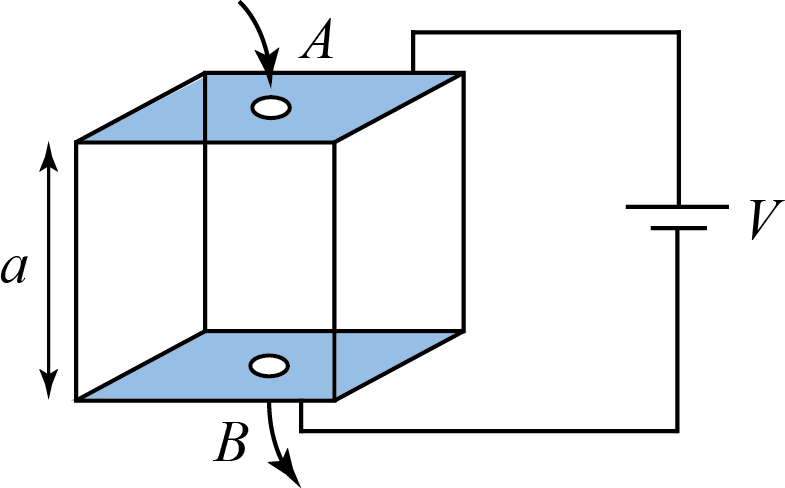
\includegraphics[height=5.5cm]{fig_3.png}
    \caption{Configuración Problema 3}
    \label{fig:fig_3}
\end{figure}
